\tikzstyle{feuille}=[]
\tikzstyle{noeud}=[]
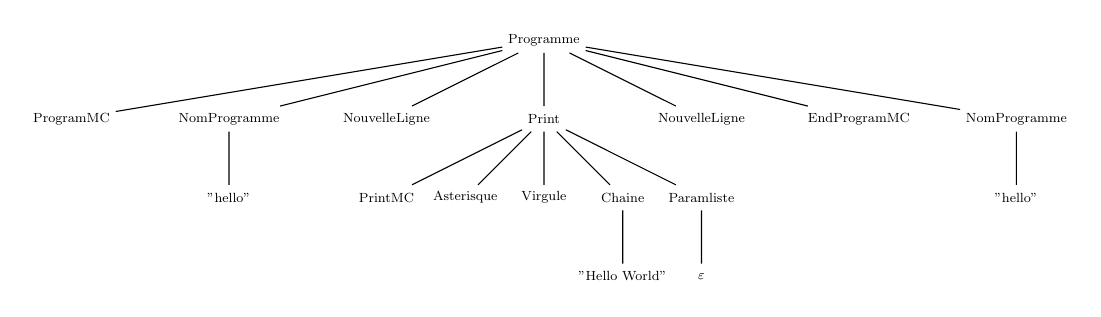
\begin{tikzpicture}
    [
        baseline=(0), 
        level/.style={sibling distance = 2cm/#1, level distance = 1cm},
        every node/.style={scale=0.6, font=\footnotesize, minimum width=15pt, minimum height=15pt}
    ]
    
    \node at (0, 0) { };
    \begin{scope}[shift={(5, 0)}]
        \node {Programme}
            child {node (0) {ProgramMC}}
            child {node (1) {NomProgramme}
                child {node (2) {"hello"}}
            }
            child {node {NouvelleLigne}}
            child {node {Print}
                child {node (3) {PrintMC}}
                child {node (4) {Asterisque}}
                child {node (5) {Virgule}}
                child {node (6) {Chaine}
                    child {node {"Hello World"}}
                }
                child{node (7) {Paramliste}
                    child {node (8) {$\varepsilon$}}
                }
            }
            child {node {NouvelleLigne}}
            child {node (9) {EndProgramMC}}
            child {node (10) {NomProgramme}
                child {node (11) {"hello"}}
            }
        ;
        \only<2>{\foreach \step in {0,1,...,11}{\drawcross{\step}}}
    \end{scope}
\end{tikzpicture}